\chapter{本研究の要素技術}
\label{tech}

本章では,本研究の要素技術となるShellとHoneypotと時系列データの扱いについて各々整理する.

\section{Honeypot}

使われているデバイスへの不正なSSHによって侵入された際,実際に攻撃が行えない環境へとフォワードし,その中で攻撃を試行させ,侵入者のログを収集する手段としてHoneypotがある.SSHのHoneypot\cite{honeypot}は低対話型Honeypotと高対話型Honeypotの大きく二種類に分けることができる.\\
%以下に侵入者がSSHで不正に機器に侵入してから踏み台にして他の機器に攻撃を仕掛けるまでの一般的なフローを図2に示す.
%\vspace{10mm}
%\begin{figure}[H]
%    \centering
%    \includegraphics[width=1.0\textwidth]{figures/nagare.png}
%    \caption{不正なSSH侵入者の想定行動フロー}
%    \label{fig:evo}
%\end{figure}


\subsection{低対話型Honeypot}
\label{tech:LowInteractionHoneypot}

SSHの低対話型Honeypotは実際のShellの挙動をエミュレートしたアプリケーションである.実際のShellの挙動をエミュレートしただけのアプリケーションなので,脆弱性がアプリケーション内に限られる.そのため,root権限を侵入者に許してしまい,踏み台にされてしまうなどの危険が極めて少ない.しかし,エミュレーションには限界があるため,コマンドやその挙動について,実際のShellとは異なる挙動をすることがある.そのため,侵入者に侵入先がHoneypotであると検知されてしまう.検知されることで,攻撃者は実際の攻撃を行わず,本来取れるはずの攻撃ログが収集できない可能性を含んでいる.そのため,収集ログの精度に問題がある.

\subsubsection{Kippo}
\label{tech:Kippo}

Kippoは,悪意のあるSSHのログイン試行者や侵入者の挙動やログを記録するために使用されるPythonで実装されたSSHの低対話型Honeypotである\cite{kippo}.Kippoは前身のKojoney\cite{kojoney}に大きく影響を受けている.ネットワークはTwisted\cite{twisted}というフレームワークで組まれている.Kippoのプロジェクトは低対話型Honeypotとして2009年に登場し,Raspberry Pi\cite{rasp}などを筆頭としたシングルボードコンピュータ\cite{singleboard}の普及と相まって広く設置された.
Kippoの機能の特徴としては収集したコマンドログ を時系列データとして保存されており,"playlog"というKippo内にあるプログラムを実行することで,過去のコマンドログ を実際にタイピングしてるかのように出力できる.また,侵入者によってダウンロードされたファイルも実行ができないように保存できる.Kippoは後述のCowrieの後継実装である.\cite{kippowiki}
KippoはIoTデバイスの高度化広く設置されたSSHの低対話型Honeypotのうちの一つであったが,実装されているコマンドも17\cite{kippocommand}と少なく,またKippo特有の異常な挙動が存在するなどと多くの問題があった.

\subsubsection{Cowrie}
\label{tech:Cowrie}
CowrieはPythonで実装されたSSHの低対話型Honeypotであり,実装はKippoのコマンドの拡張や,攻撃者がリダイレクトでマルウェアを送り込む手法をとって送り込んだマルウェアを収集可能にしたりするなど,様々な機能を拡張したものである.
Kippo特有の異常な挙動を改善しており,実装コマンド数は38\cite{cowriecommand}とKippoより少し多くなっているものの\cite{differfromkippo},Cowrie特有の異常な挙動もまだまだ多い.

%\subsection{製造責任と知的財産権に関する法制度}
%\label{tech:lows}


\subsection{高対話型Honeypot}
\label{tech:HighInteractionHoneypot}

\subsubsection{Honeynet Project}
\label{tech:Honeynet}

\subsection{SSHのHoneypotの比較}
\label{tech:CompareHoneypot}
以上をまとめたSSHの低対話型HoneypotとSSHの高対話型Honeypotの比較を行った表を図2.1に示す.

\vspace{10mm}
\begin{figure}[H]
    \centering
    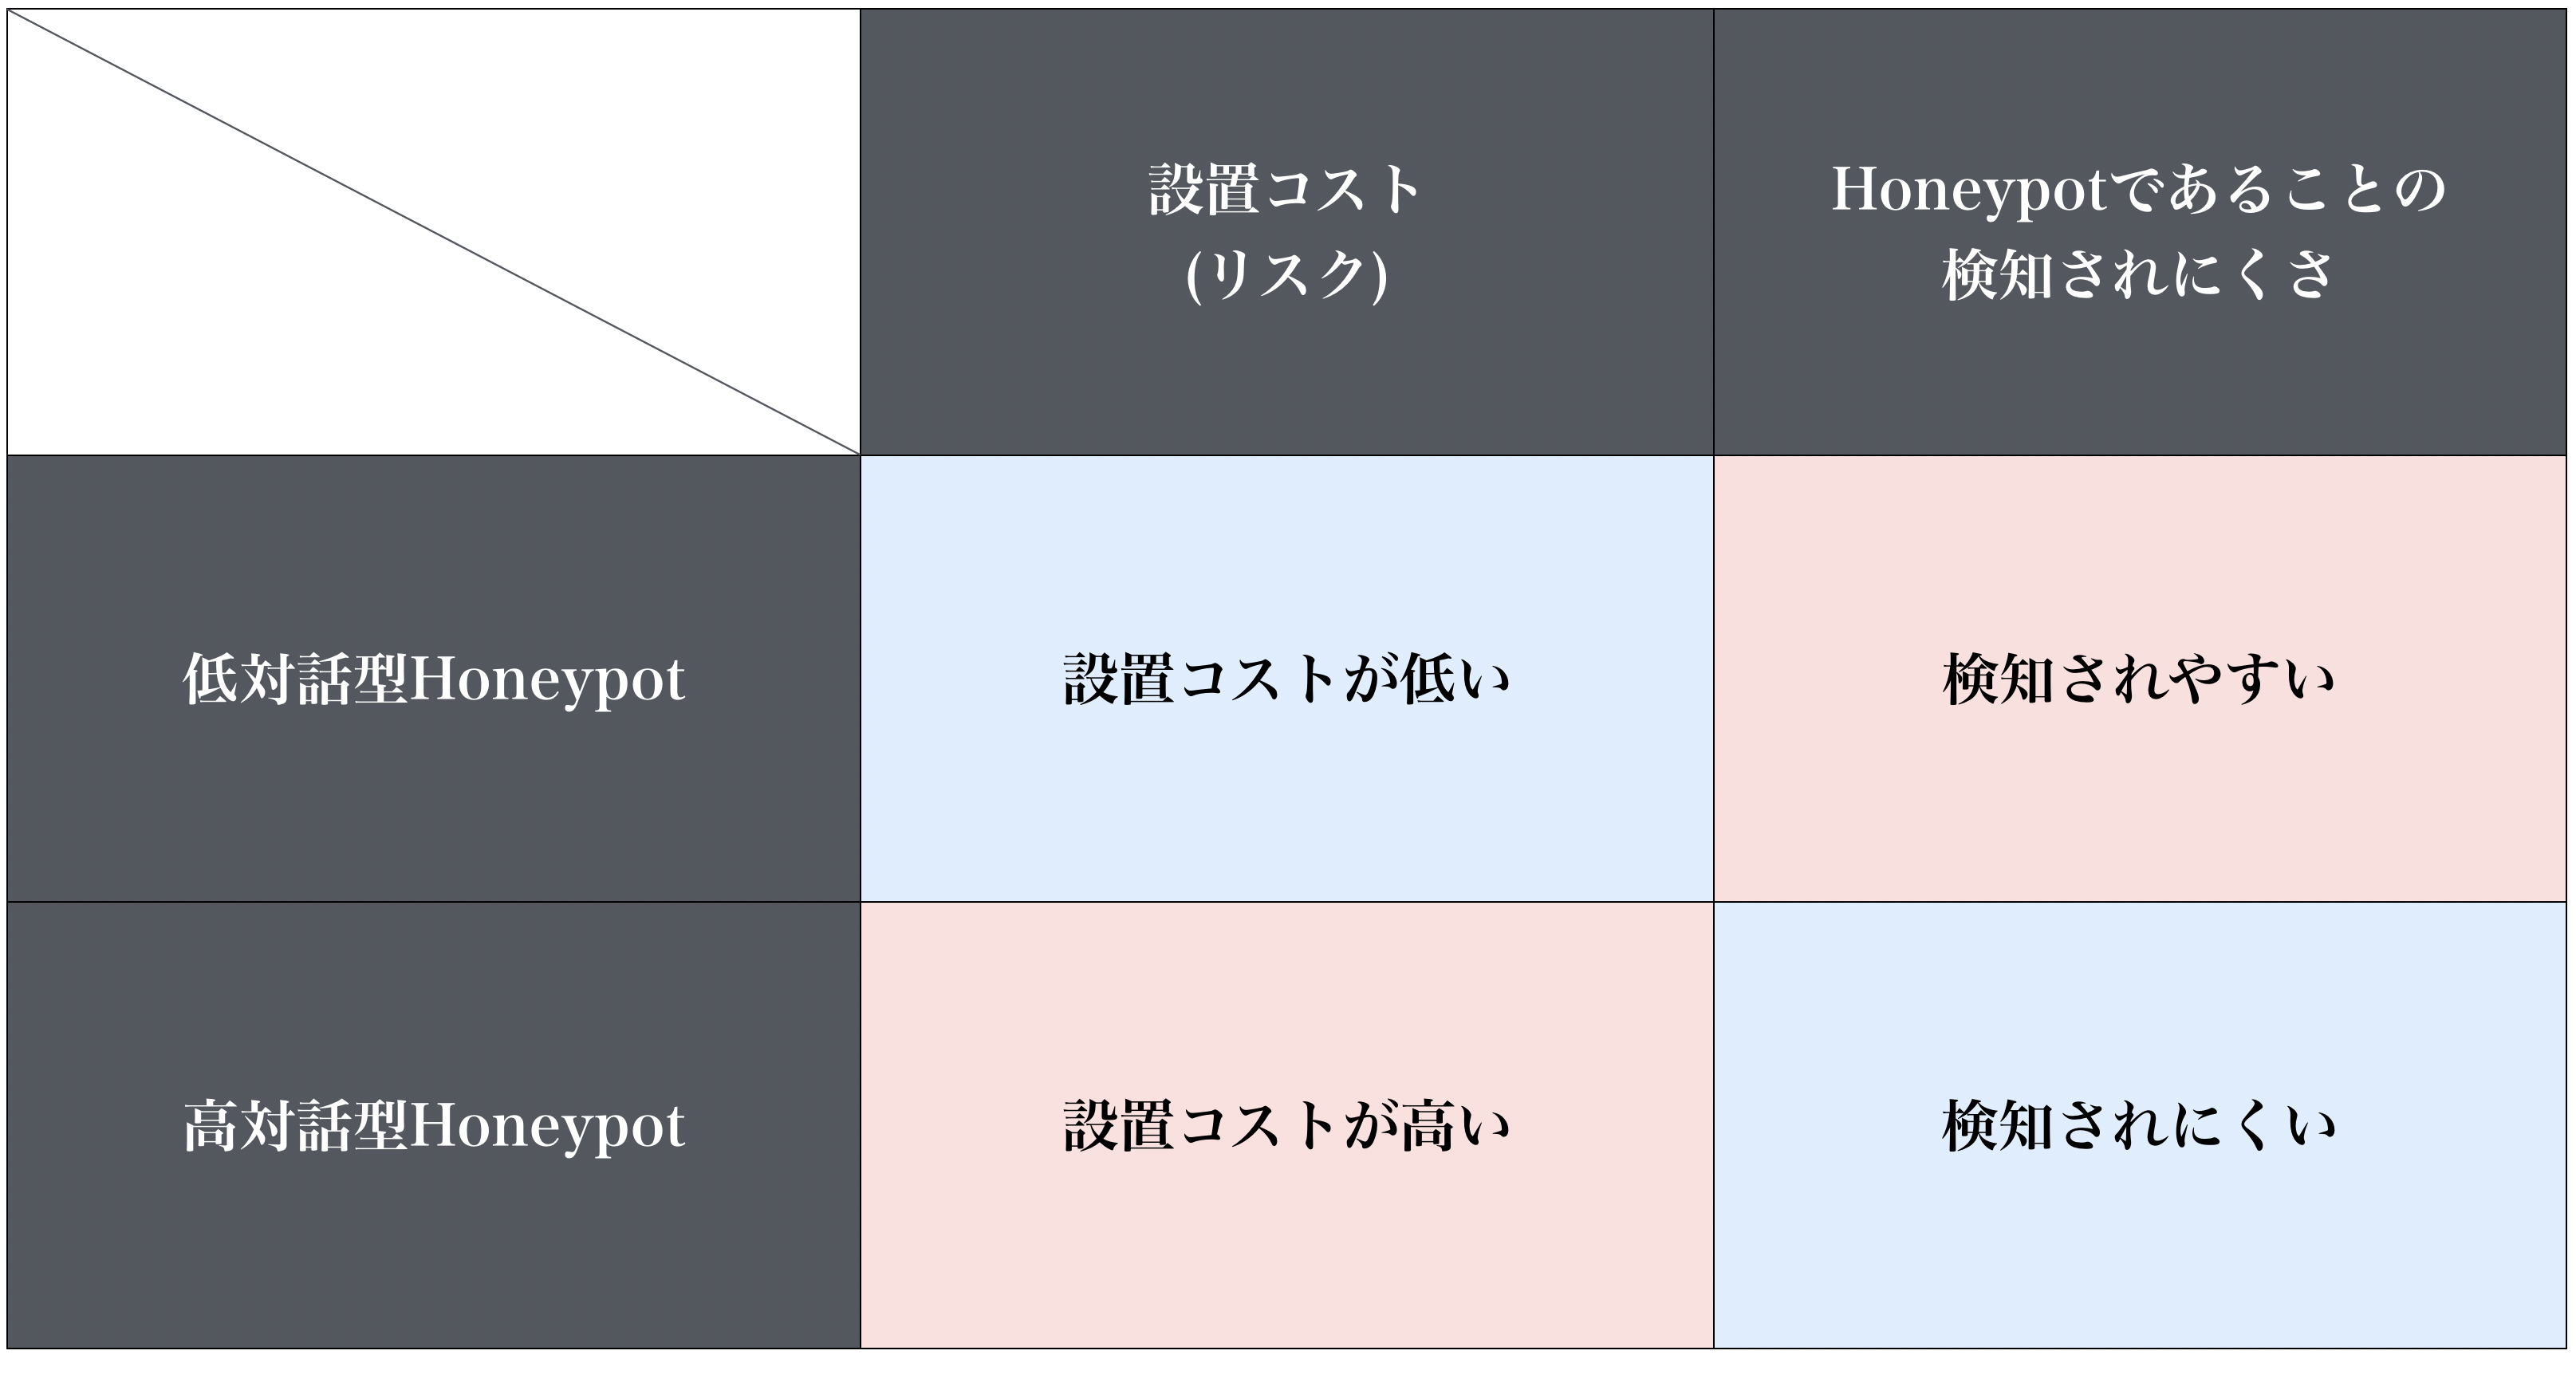
\includegraphics[width=1.0\textwidth]{figures/compare.png}
    \caption{SSHの低対話型HoneypotとSSHの高対話型Honeypotの比較}
    \label{fig:evo}
\end{figure}

%\begin{itemize}
%\setlength{\leftskip}{1.0cm}
% \item[危険責任] 製造者は製造物の設計図などの情報を消費者より詳細に知り得るため
% \item[報償責任] 製造者は製造物により利益を得るためそこから生じる責任を負うべきである
% \item[信頼責任] 製造者は自己の製品の安全性についてPRしており消費者はその品質が担保されているものであると期待する
%\end{itemize}

\section{Shell}
\label{tech:Shell}
ShellはOSのユーザーのためにインタフェースで,カーネルのサービスへのアクセスを提供するソフトウェアである.本研究での"Shell"はコマンドラインシェルのことを指す.

\subsection{Secure Shell}
\label{tech:Secure Shell}
Secure Shell(セキュアシェル、SSH)は、暗号や認証の技術を利用して、安全にリモートコンピュータと通信するためのプロトコルである.パスワードなどの認証部分を含むすべてのネットワーク上の通信が暗号化される.\cite{ssh}SSHにおける問題としては,通信する上での認証方法には鍵認証を推奨されているが,デフォルトではパスワード認証になっている.パスワード認証のままだとパスワードの総当たり攻撃を受けたり,パスワードが標準のままの設定であることで不正なログイン試行によって侵入を許してしまう.

\subsection{BusyBox}
\label{tech:BusyBox}
BusyBoxは標準UNIXコマンドで重要な多数のプログラムを単一のバイナリファイルに含むプログラムである.BusyBoxに含まれる,多数の標準UNIXコマンドで必要とするプログラムの実行ファイルは,LinuxというOSをBusyBoxだけでディストリビューションできるよう,"Linux上で最小の実行ファイル"として設計されている.一般にインストールされる実行ファイルは一部だけを実装できるように選択することができる.一般的にはBusyBoxのコマンドは200以上も用意されている.\cite{busybox}\footnote{今回使用したBusyBoxに含まれるコマンドの数は219}.
BusyBoxをインストールして実際に各コマンドを実行するためには,BusyBox内にある各コマンドにアクセス可能なようにpathを通すだけで良い.

\section{自然言語処理}
\label{tech:NLP}
人間が日常的に使っている自然言語をコンピュータに処理させる一連の技術である.本研究において,自然言語処理は意味解析のために使用した.意味解析には様々な手法があり,現在では大きくシソーラス解析とベクトル空間分析がある.

\subsection{シソーラス解析}
\label{tech:Siso}
シソーラスとは単語を意味レベルで分解し,抽象度の高いものから低いものへと遡っていくことができ,それを体系づけた類語辞書のことである.シソーラスには様々な言語において有名な辞書が存在する.有名なシソーラスとしてはPrinceton UniversityのWordNetがある.\cite{wordnet}

\subsubsection{Wordnet}
\label{tech:Wordnet}
WordNetは英単語がsynsetと呼ばれる同義語のグループに分類され,簡単な定義や,他の同義語のグループとの関係が記述されているデータベースである.WordNetのデータベースは約11万5000のsynsetに分類された約15万語を収録し,全体で20万3000の単語と意味の組み合わせがある.\cite{wordnetwiki}

\subsection{ベクトル空間解析}
\label{tech:Vector}
単語の意味を表現するため,単語の文章での出現回数や,その単語の周辺の単語をマトリクス上に表現することで,その単語を数学的に解釈できるようにしている.

\subsubsection{ベクトル空間モデル}
\label{tech:voctorkukan}
ベクトル空間モデルとは文章を多次元空間上にベクトルとして表現し,それぞれのベクトルの比較を行うことで類似度を算出するためのモデルである.文章の類似度が高いほどベクトルの方向が近いということなので,比較した文章のベクトルのなす角が小さければ文章の類似度が高いということになる.\\
m個の単語が使用されている文章dにおける各単語の重要度を$ w_{d1},w_{d3},w_{d3}, \ldots ,w_{dm} $とすると,文章dのベクトルは以下のように表される.
\vspace{1mm}
\[
\vec{d} = (w_{d1},w_{d3},w_{d3}, \ldots ,w_{dm})
\]
\vspace{1mm}
また,同様にしてn個の単語が使用されている文章eをベクトル表現すると,
\vspace{1mm}
\[
\vec{e} = (w_{d1},w_{d3},w_{d3}, \ldots ,w_{dn})
\]
\vspace{1mm}
と表すことができる.
したがって,$ \vec{d} $ と $ \vec{e} $のなす角$ \theta $における$ \cos \theta $は以下のように表される.
\vspace{2mm}
\[
\cos \theta = \frac{\vec{d} \cdot \vec{e}}{|\vec{d}| |\vec{e}|}
\]
\vspace{2mm}
ベクトル化した時の単語の重要度はTF-IDFのアルゴリズム(※~\ref{tech:tfidf})を用いて算出した重みを用いることで,これを表すことができる.~\cite{voctormodel}

\subsubsubsection{TF-IDF}
\label{tech:tfidf}
TFとはTerm Frequencyのことで,文章内での単語の出現頻度を表す.
数式では以下のように表される.
\vspace{3mm}
\[
tf(t,d) = \frac{n_{t,d}}{\sum_{s \ni{d}}n_{s,d}}
\]
\vspace{5mm}
$ tf(t,d) $はTFの値で,文章d内に含まれる単語tの出現頻度を表す.\\
$ n_{t,d} $は文章dにおける単語tの出現回数を表す.\\
$ \sum_{s \ni{d}}n_{s,d} $は文章dにおける全ての単語の出現回数を表す.\\
以上を踏まえTFの値とは,
\vspace{2mm}
\[
\mbox{文章d内に含まれる単語tの出現頻度} = \frac{\mbox{文章dにおける単語tの出現回数}}{\mbox{文章dにおける全ての単語の出現回数}}
\]
\vspace{2mm}
を数式で表したものである.\\
IDFとはInverse Document Frequencyのことで,ある単語が様々な文章においてどれほど使われているのかを表す.
数式では以下のように表される.
\vspace{2mm}
\[
idf(t) = \log{\frac{N}{df(t)}+1}
\]
\vspace{2mm}
$ idf(t) $はIDFの値で,単語tが全文章数Nでどれほど使われているのかを表す.\\
$ N $は全文章数を表す.\\
$ df(t) $は単語tが出現する文章の数を表す.\\
以上を踏まえIDFの値とは,
\vspace{2mm}
\[
\mbox{単語tが全文章数Nでどれほど使われているのか} = \frac{\mbox{全文章数}}{\mbox{単語tが出現する文章の数}+1}
\]
\vspace{2mm}
を数式で表したものである.\\
このようなTFの値とIDFの値を重みとすることで,文章を特徴付ける単語の抽出をするものがTF-IDFである.


\subsubsection{word2Vec}
\label{tech:word2vec}
word2vecは2層からなるニューラルネットワークである.word2vecには2つのアーキテクチャがあり,一つは$ Continuous Skip-gram Model $,もう一つは$ Continuous Bag-of-Words Model $である.$ Continuous Skip-gram Model $は入力に文章中の任意の単語を用意し,出力に文章においてその任意の単語の前後の周辺語を用意し,ニューラルネットワークに読み込ませることで第一層から第二層への重みを獲得することが目的である.$ Continuous Bag-of-Words Model $では逆に出力に文章中の任意の単語を用意し,入力に文章においてその任意の単語の前後の周辺語を用意し,同様にしてニューラルネットワークに読み込ませることで第一層から第二層への重みを獲得することが目的である.本研究ではより精度の高い$ Continuous Skip-gram Model $(以降,$ Skip-gram Model $と呼ぶ.)を使用した.\cite{word2vecpaper}

\subsubsection{Continuous Skip-gram Model}
\label{tech:skipgram}
$ Skip-gram Model $は先述の通り,与えられた単語に対してその周辺語を予測するためのモデルのことである.このモデルは2層からなるニューラルネットで,入力にはOne-hotベクトルを用いる.One-hotベクトルとは$ (0,0,0, \ldots ,1, \ldots ,0) $のように,単語のインデックスから抽出する単語だけを$ 1 $と表記することで表現するベクトルのことである.\\
入力層から隠れ層への重みは$ V \times N $のマトリクス$ W $で表され,Wの各列は単語ベクトルとなっている.隠れ層から出力層への重みはマトリクス$ W $を転置した$ N \times V $のマトリクス$ W^{\prime} $となっている.\\
このようなモデルを条件付き確率で表現すると,
\[
p(w_{O}|w_{I}) = \frac{exp({v^{\prime}^{\mathrm{T}}_{W_{V}}} \cdot v_{w_{I}})}{\sum_{W_{v} \in{V}}exp({v^{\prime}^{\mathrm{T}}_{W_{V}}} \cdot v_{w_{I}})}
\]
と表せる.


%%% Local Variables:
%%% mode: japanese-latex
%%% TeX-master: "../bthesis"
%%% End:
